
\section{Introduction {\normalfont (3 pages) [Christian]}}

``The fundamental problem of star formation is how stars accrete their mass.'' \citep{Dunham_2014}.


How did the Sun form, how the Earth? Answering these questions requires the identification and study of the Sun's progenitors,  young stellar objects that will evolve into a stellar system like ours. Therefore, we primarily discuss stellar systems broadly resembling the young Sun's, i.e., with stellar masses below about 2$\,M_\odot$.

Such stars and planets form in molecular clouds, often associated with filaments within the clouds,  where denser, cooler parts collapse. In these regions, gravity dominates over the stabilizing effects of thermal pressure, turbulence, and magnetic fields \citep[e.g., ][]{McKee_2007} and protostars form  \citep{Andre_2014}. The first, self-gravitating, hydrostatic core contains only a small fraction of the final stellar mass ($\sim0.01\,M_\odot$) and most of the mass still in the envelope \citep[e.g.,][]{Gong_2015,Lee_2020}; these objects are called class~0 objects \citep[see Fig.~\ref{fig:starform_classes} top left, and ][]{Andre_1993, Larson_2003}. Due to angular momentum conservation, a disk forms around the central condensation and outflows are launched, which regulate the angular momentum balance of the system. The collimated outflows, jets, propagate into the interstellar medium beyond the envelope and are often the first detectable signs of a forming star. After disk formation, accretion proceeds through the disk onto the protostar while enevelope material falls onto the disk \citep{Padoan_2014}. Eventually, the protostar's mass equals the envelope mass after roughly $10^5$\,yrs and the objects are called class~{\sc i} objects (Fig.~\ref{fig:starform_classes} top right), they are also hotter and more luminous than class~0 objects. It is believed that planet formation sets in during the class~I stage \citep{}.

Eventually, the envelope disperses and the young stellar object (YSO) becomes visible at optical wavelengths at a stellar age of $\sim1\,$Myr. The dispersal mechanism is not clear yet, but winds and radiation from nearby OB stars if present or otherwise radiation and outflows from low mass stars likely play a major role. Also the (wide-angle) winds launched by the forming stellar system itself may contribute to the envelope dispersal and to reduce the envelope to star mass conversion efficiency of to one third \citep{Frank_2014}. Accretion then proceeds from the disk in these class~{\sc ii} sources or classical T~Tauri stars. Planet formation is already ongoing during this stage of star formation and we get a first relatively unobscured view to the newborn stars (Fig.~\ref{fig:starform_classes} bottom left).

\begin{figure}[t]
\centering
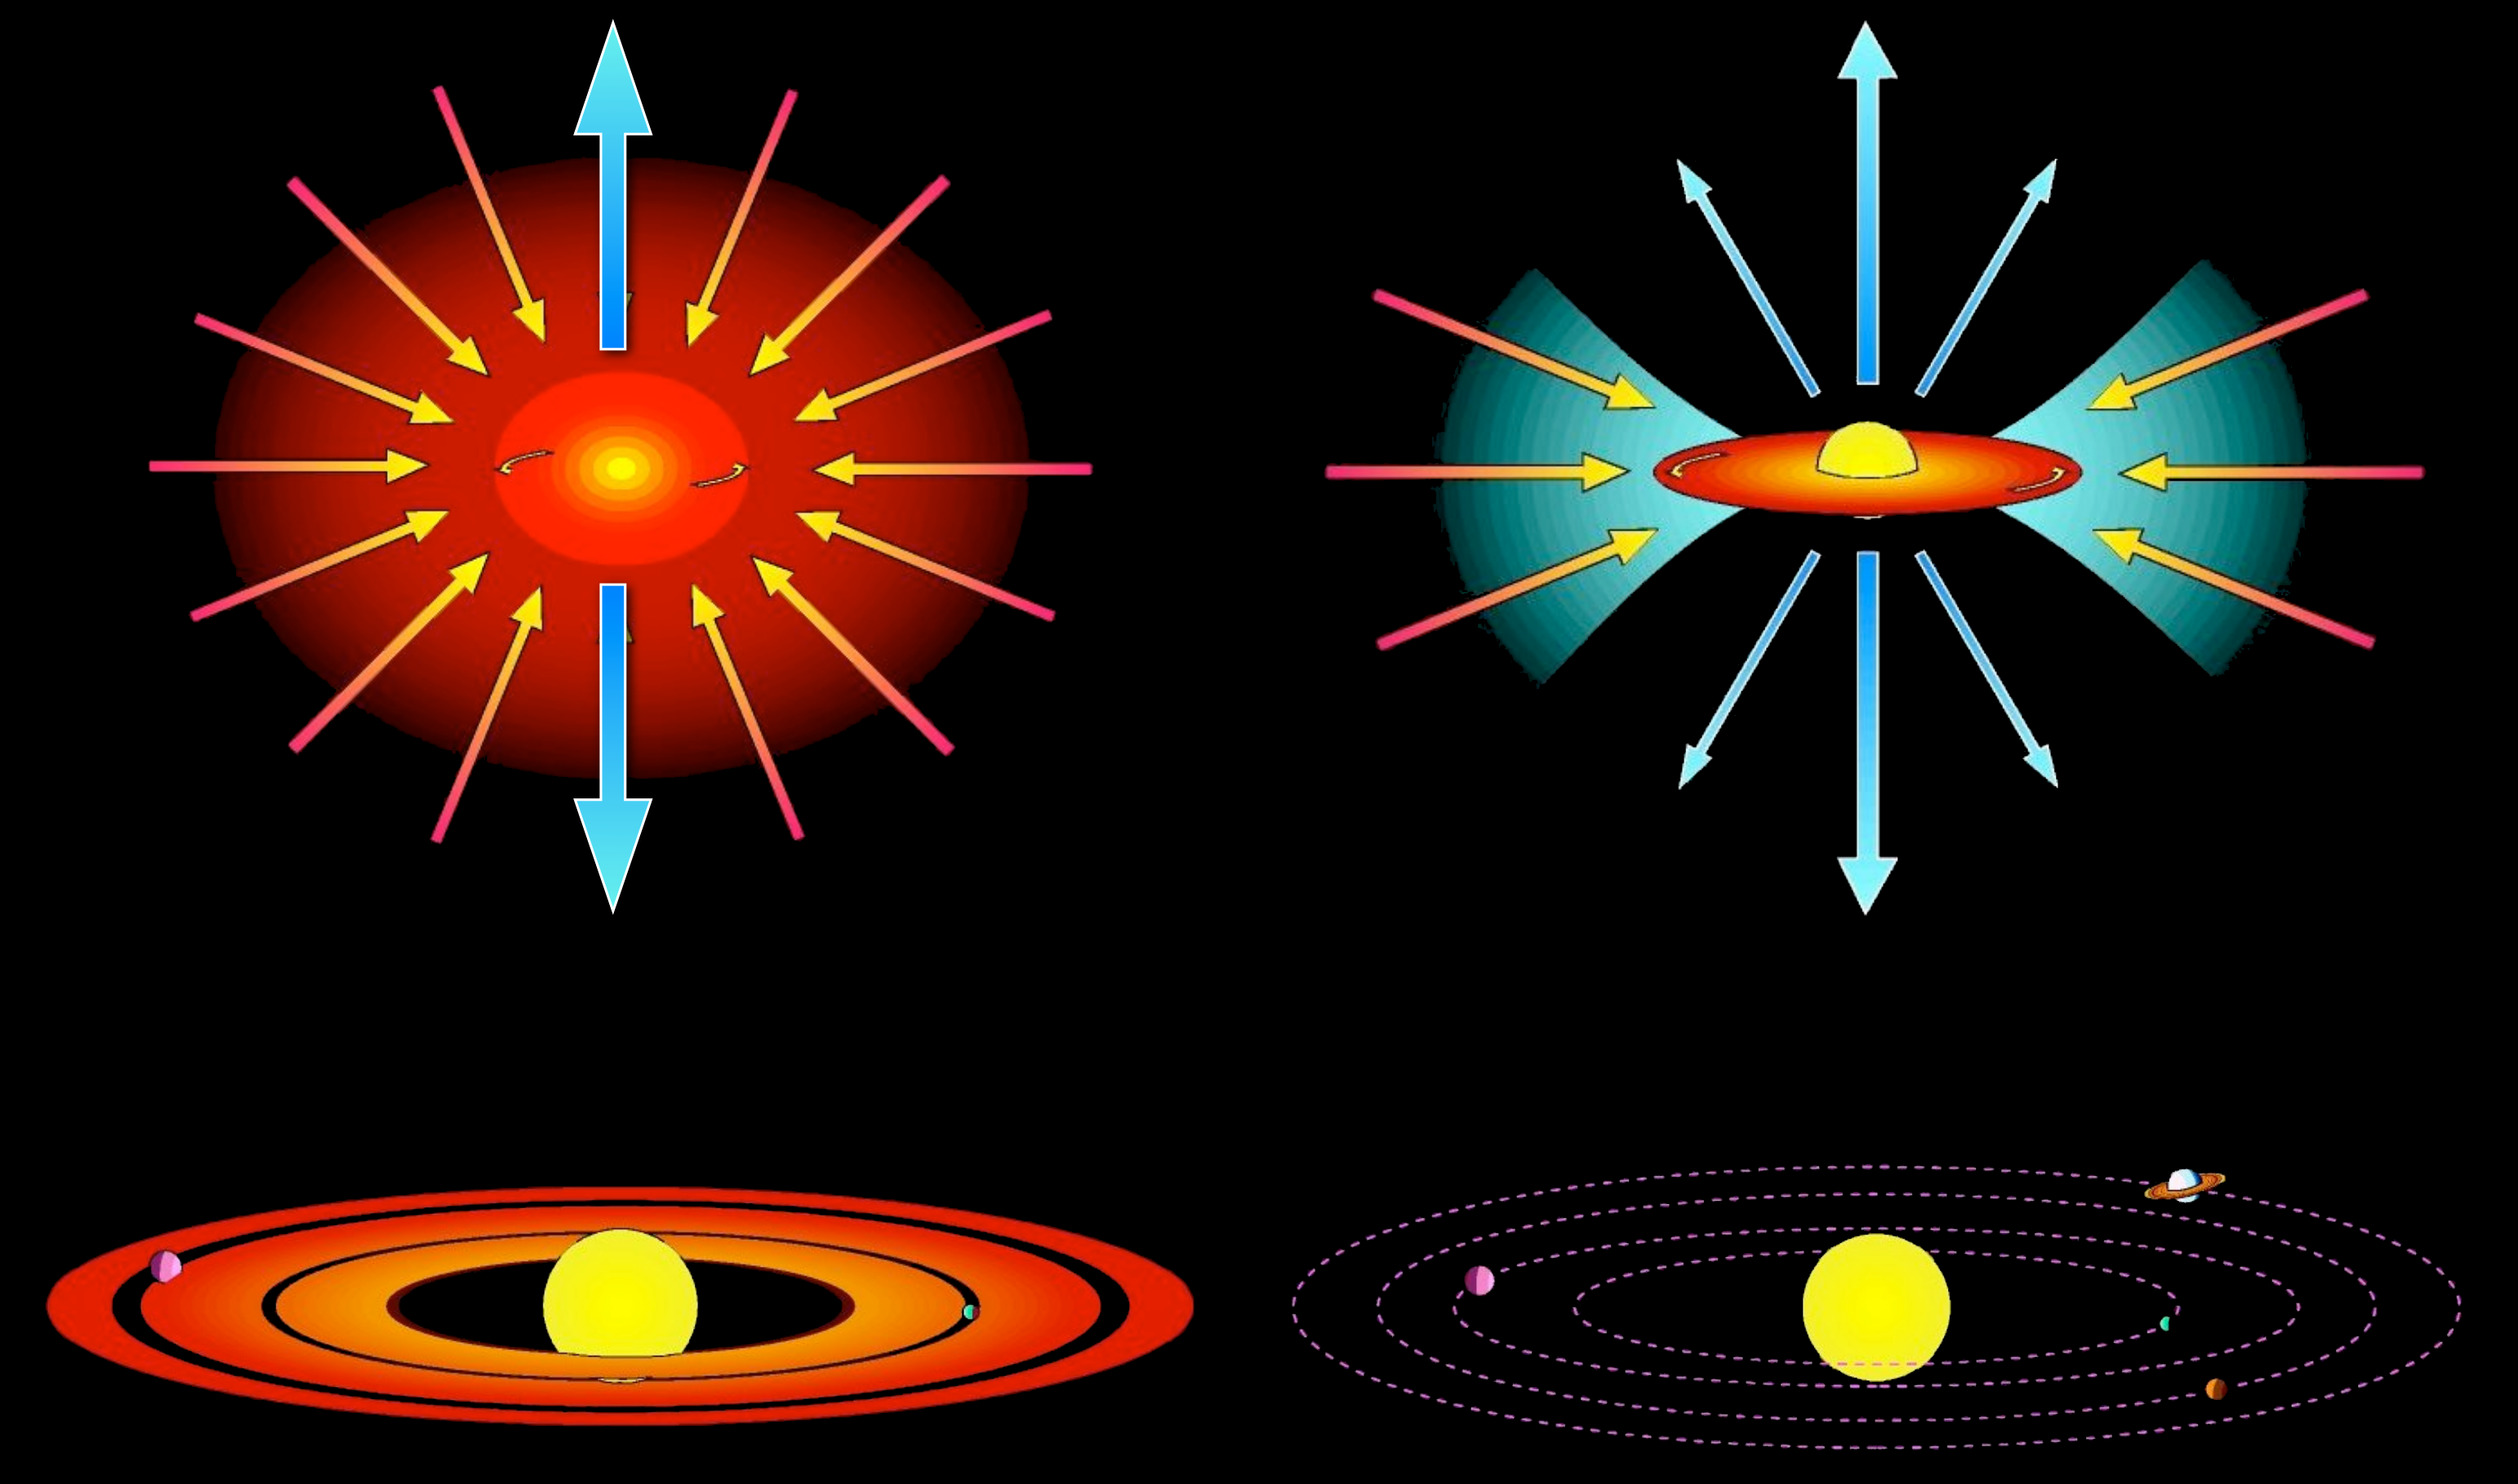
\includegraphics[width=10cm]{figs/starform_classes.png}
\caption{Star formation sequence. Adapted from original diagram by M.~McCaughrean. \label{fig:starform_classes}}
\end{figure}

Finally, the disk dispersed, too, after another few Myrs leaving behind a pre-main sequence star, perhaps surrounded by planetary system, which slowly contracts towards it's  main-sequence radius (Fig.~\ref{fig:starform_classes} bottom right). Solar mass stars take approximately 100\,Myrs to reach the main sequence where they reside for over 10\,Gyr.

Within this sequence of star formation, the classical T~Tauri star phase stands out, because the relatively unobscured view towards the central region around the forming stars provides us with the most detailed picture of the physical processes, including planet formation, using a large variety of observational techniques including X-ray data.

\subsection{T Tauri Stars}
T~Tauri stars were first described as a distinct class of objects  by \citeauthor{Joy_1945} in 1945 based on their pronounced optical variability \citep{Joy_1945}. The notation that T~Tauri stars are young came with the realization that they are located to the top right of  main sequence (MS) stars in the Hertzsprung-Russel diagram (HRD), consistent with the expected position of stars contracting along their Hayashi tracks towards the MS \citep{Hayashi_1961}. Also , strong Li absorption lines suggest a young age, because  Li is quickly depleted in stellar photospheres \citep{Magazzu_1992}.


\begin{figure}[t]
\centering
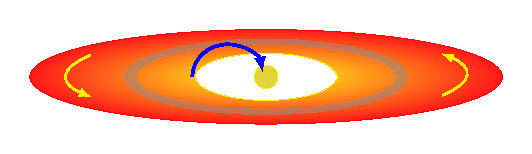
\includegraphics[width=10cm]{sketches/ctts.pdf}
\caption{Sketch of a classical T~Tauri system. \label{fig:ctts_sketch}}
\end{figure}


The physical processes that cause other prominent features seen in the so-called classical T~Tauri stars (CTTSs), however, remained controversial.
For example, there was no consensus on the origin of the
strong emission lines like H$\alpha$, termed “chromospheric emission”, until the 1980s when the infrared excess of CTTSs was discovered and correctly ascribed to cold dusty disks around the central star. Also, the discovery that the ``chromospheric'' line profiles change from inverse to normal P~Cygni profiles and back within few days on individual systems helped to converge on a scenario in which accretion shocks and outflows are the main processes for explaining CTTS features \citep[as nicely described in][]{Bertout_2007}, in addition to their protoplanetary disks.

Disks, accretion, and outflow are still the processes that define the properties of CTTS. Figure~\ref{} shows a sketch of a T Tauri system.
During the CTTS phase, the stellar mass is already close to the final stellar mass but the interior is fully convective \citep{}, which together with rather rapid rotation (few days) leads to a strong stellar dynamo \citep{}. Stellar magnetic fields during the CTTS phase are therefore in the kG range \citep{}. Such strong magentic fields disrupt the disk close to the star, that is within a few stellar radii, as the star, being hydrostatic, rotates slower than an approximately Keplerian disk. The interaction of the stellar magnetic field with the inner parts of the disk slows the innermost disk material down so that it cannot resist gravity anymore and is channeled along the stellar magentic field lines onto the star. Travelling along the magnetic field line, the matieral is accelerated to almost free-fall velocity and impacts the stellar photosphere where a strong shock forms. The details of the accretion shock are described in sect.~\ref{sect:accretion}.%, briefly the shock velocities are on the order of 300\,km\,s$^{-1}$ resulting in post shock temperatures in the $10^6$\,K range and, thus, radiative cooling of the post shock plasma causes X-ray emission.

The inner disk would be depleted within $10^3$ to $10^4$ years without being replenished by material from outer disk radii. Therefore, continued accretion requires radial transport of material through the disk, from outer to inner disk radii. Radial transport through the disk requires the redistribution of angular momentum (AM) and several processes have been invoke to promote this AM redistribution, prominent examples include the magneto-rational instability \citep[MRI,][]{Balbus_1991} with non-ideal MHD extensions and disk winds \citep{Blandford_1982, Pudritz_1983}, again with the inclusion of non-ideal MHD effects. In reality, the vertical structure of protoplanetary disks likely results in different transport mechanisms dominating at different disk heights with most of the mass being transported through the upper disk layers where also magnetro-centrifugally driven winds are launched.

Magneto-centrifugally launched winds require some net vertical magnetic field threading the disk. Material is accelerated along magnetic field lines until the magnetic field strength becomes insufficient to control the particle motion and the Lorentz force causes the collimation of the outflowing material into narrow jets. The jet velocity depends on the so-called magnetic lever arm, which relates the Keplerian velocity at the launch radius to the jet velocity and is of order 10 \citep{}; hence, jet velocities are on the order of 300\,km\,s$^{-1}$. In addition to disk winds, there may be other outflows like stellar winds, magneto-spheric ejections (from the star or the star-disk interaction region), or the so-called X-winds from the inner disk edge \citep{Shu_}. 

At some point, typically after a few Myrs, the disk has dispersed \citep{} and we are left with a pre-main sequence star with a number of orbiting planets, such objects are call weak-line T~Tauri stars (WTTSs). 

\subsection{The power of X-rays for studying T~Tauri stars}
The different parts of a classical T~Tauri system have grossly different temperatures: The disk midplane may be characterized by only few 10~K, the upper disk layers are likely above 1000~K, the inner edge of the disk is typically assumed to be around 2\,000~K, and we typical stellar photospheric temperatures are 3-4\,000~K. Therefore, the intrinsic emission of these different components peaks in very different wavebands, which is reflected in the observational tools used to study them, sub-mm radio to IR observations enjoy great popularity for disk studies while optical to NIR data are powerful for studying the more dynamic processes such as accretion and outflows. There are, however, some interesting exceptions, e.g., FUV data probe the hydrogen content of the inner disk as well as accretion \citep[see review by][]{Schneider_2020}.

On first sight, it may therefore appear surprising that X-ray observations play an important role for studying CTTS. However, a flow with velocities in excess of 300\,km\,s$^{-1}$, like the accretion flow or the jet, which rams into a stationary obstacle shock heats the post to temperatures in excess of 1\,MK  so that radiative cooling of such a plasma causes X-ray emission so that X-ray studies of CTTSs (and younger objects for the outflow case) probe the (in- and out-) flow properties. 

X-ray data is even powerful for studying disk properties using transmission spectroscopy. Extinction at optical wavelengths\footnote{Strictly radiation with wavelengths longer than the 912\,\AA{}, the Lyman limit of hydrogen.} is dominated by dust grains while X-rays are absorbed by gas and dust. The ratio of X-ray to optical extinction therefore depends on the absorber's gas-to-dust ratio, which has been beneficially used using transmission spectroscopy of near edge-on protoplanetary disks \citep{}. Lastly, T~Tauri stars are rapidly rotating and so are also strong X-ray emitters (see chapter by J.~Kastner).
